% This must be in the first 5 lines to tell arXiv to use pdfLaTeX, which is strongly recommended.
\pdfoutput=1
% In particular, the hyperref package requires pdfLaTeX in order to break URLs across lines.

\documentclass[11pt]{article}

% Add the "review" option to enable line numbers for reviewing.
\usepackage{ACL2023}

% Standard package includes
\usepackage{times}
\usepackage{latexsym}

% For proper rendering and hyphenation of words containing Latin characters (including in bib files)
\usepackage[T1]{fontenc}
% For Vietnamese characters
% \usepackage[T5]{fontenc}
% See https://www.latex-project.org/help/documentation/encguide.pdf for other character sets

% This assumes your files are encoded as UTF8
\usepackage[utf8]{inputenc}

% This is not strictly necessary, and may be commented out.
% However, it will improve the layout of the manuscript,
% and will typically save some space.
\usepackage{microtype}

% This is also not strictly necessary, and may be commented out.
% However, it will improve the aesthetics of text in
% the typewriter font.
\usepackage{inconsolata}

% Additional packages for figures and graphics
\usepackage{graphicx}
\usepackage{amsmath}
\usepackage{booktabs}
\usepackage{tabularx}
\usepackage{enumitem}
\usepackage{hyperref}
\usepackage{pgfplots}
\usepackage{tikz}
\usepackage{tikzstyles}  % Our custom TikZ styles

% Configure pgfplots
\pgfplotsset{compat=1.17}


% If the title and author information does not fit in the area allocated, uncomment the following
%
%\setlength\titlebox{<dim>}
%
% and set <dim> to something 5cm or larger.

\title{MovieQA-RAG: A Modular RAG Framework with Metadata-Guided Retrieval and Explainable Evaluation}

% Author information can be set in various styles:
% For several authors from the same institution:
% \author{Author 1 \and ... \and Author n \\
%         Address line \\ ... \\ Address line}
% if the names do not fit well on one line use
%         Author 1 \\ {\bf Author 2} \\ ... \\ {\bf Author n} \\
% For authors from different institutions:
% \author{Author 1 \\ Address line \\  ... \\ Address line
%         \And  ... \And
%         Author n \\ Address line \\ ... \\ Address line}
% To start a separate ``row'' of authors use \AND, as in
% \author{Author 1 \\ Address line \\  ... \\ Address line
%         \AND
%         Author 2 \\ Address line \\ ... \\ Address line \And
%         Author 3 \\ Address line \\ ... \\ Address line}

\author{Sajjad Hossain, Mahmudul Hassan Navid, Md Zahidul Islam, Nuri Jannatul \\
  International Software Systems Science \\
  Otto-Friedrich-University Bamberg}

\begin{document}
\maketitle
\begin{abstract}
This paper presents an enhanced Retrieval-Augmented Generation (RAG) system for movie question-answering and recommendation. We introduce three key enhancements: (1) metadata filtering for targeted retrieval, (2) query normalization for linguistic variations, and (3) comprehensive evaluation analytics. Our system processes heterogeneous movie data from multiple CSV sources, combining structured attributes with plot overviews to support diverse query types, from factual questions to analytical computations. The modular pipeline integrates data transformation, chunking, embedding storage, and enhanced query parsing that normalizes temporal and categorical constraints. Our evaluation framework employs 84 gold-standard questions across four difficulty levels, with multi-dimensional metrics tracking retrieval accuracy, answer quality, and performance stability. Key contributions include effective metadata parsing, query normalization techniques, multi-faceted retrieval combining semantic search with metadata filtering, and a stratified evaluation methodology.
\end{abstract>

\section{Introduction}

Our enhanced RAG system enables natural language question-answering and recommendation for movie databases. Users can query diverse movie attributes including budget, revenue, cast, genres, production details, and plot content through conversational interfaces. The system supports factual retrieval (``\textit{Who produced Pinocchio?}'') and analytical queries (``\textit{Which movies under \$10M budget earned more than \$500M revenue? Include ROI calculation.}''). Movie recommendation leverages plot similarity and user preferences, addressing scenarios requiring intelligent movie information access without structured query knowledge.

\subsection{Problem Statement}
Existing movie information systems inadequately handle natural language queries requiring correlation across heterogeneous data sources. We address three core challenges: (1) effective processing and integration of multiple CSV movie datasets with varying schemas, (2) handling linguistic variations and temporal constraints in user queries, and (3) maintaining retrieval accuracy for both semantic content matching and structured metadata filtering. Traditional approaches either focus exclusively on text similarity or require structured queries, failing to bridge natural language understanding with multi-attribute movie data analysis.

\subsection{Motivation}
Movie information systems face a fundamental mismatch: users ask questions like "What was that thriller from the 90s with the plot twist?" while systems expect structured queries with exact field names and values. RAG bridges this gap between natural language and structured data retrieval. Movie data presents unique challenges, making RAG particularly well-suited: combining structured metadata (budgets, release dates, cast) with unstructured text (plot summaries), requiring temporal reasoning, and involving subjective attributes like genre classification. RAG's ability to handle linguistic variations becomes crucial when users express constraints differently ("movies from 1995" vs. "mid-90s films"), as the retrieval component normalizes these variations while the generation component provides coherent responses.

\begin{figure*}[!ht]
\centering
\begin{tikzpicture}

% Define fixed positions for better control
% Row 1 - Query processing
\node[process] (query) at (0,0) {User Query};
\node[process] (parsing) at (3,0) {Filter Parsing \&\\Normalization};
\node[storage] (vectorstore) at (7,0) {ChromaDB\\Vector Store};
% Using the retrievedchunks pic defined in tikzstyles.sty

% Use the custom node in your diagram
\pic[name=chunks] at (6.5,-1.85) {retrievedchunks};
\node at (7,-2.25) [font=\tiny, align=center] {Enriched\\Retrieved Documents};

% Row 2 - metadata (aligned vertically with Retrieved Documents)
\node[storage] (metadata) at (11,-1.5) {Metadata\\Sources};

% Row 3 - LLM (aligned vertically with Retrieved Documents)
\node[process] (llm) at (2,-1.5) {LLM Generation\\(GPT-4.1-nano)};
\node[io] (answer) at (0.5,-3) {Answer\\(User)};
\node[data] (insights) at (3.5,-3) {Insight\\Logging};

% Connections
\draw[arrow] (query) -- (parsing);
\draw[arrow] (parsing) -- node[above, font=\tiny] {Normalized Query} (vectorstore);
\draw[arrow] (vectorstore) -- (7,-1); % This draws FROM vectorstore TO chunks

\draw[arrow] (metadata) -- node[above, font=\tiny] {Metadata Injection} (7.75,-1.5);
\draw[arrow] (6.5,-1.5) -- (llm);
\draw[arrow] (llm) -- (answer);
\draw[arrow] (llm) -- (insights);

\end{tikzpicture}
\caption{Enhanced RAG system architecture with metadata-guided retrieval, showing the flow from user query through normalized filtering, context enrichment, and answer generation.}
\label{fig:architecture}
\end{figure*}

\section{System Description}

\subsection{Pipeline Architecture}

Our modular pipeline architecture consists of four core components:

\begin{itemize}
\setlength{\itemsep}{0pt}
\setlength{\parsep}{0pt}
\item \textbf{Raw-to-processed:} Integrates multiple CSV sources, samples $\sim$6k to $\sim$1k movies, creates structured JSON format.
\item \textbf{Processed-to-embeddings:} Generates chunks, creates embeddings, stores in ChromaDB with metadata.
\item \textbf{Evaluation:} Automates performance tracking with gold dataset and analytical insights.
\item \textbf{User query:} Real-time question-answering with enhanced retrieval and generation.
\end{itemize}

\subsection{Key Enhancements}

We implemented iterative improvements across seven evaluation cycles: stricter prompt engineering with few-shot examples, embedding model upgrade from \textbf{text-embedding-ada-002} to \textbf{text-embedding-3-small}, query normalization for linguistic variation handling, metadata injection into retrieval context, and LangChain tool calling for structured filter parsing. These enhancements address three fundamental limitations: LLM non-determinism, context-answer misalignment, and inconsistent metadata filter extraction.

\subsection{Challenges and Resolutions}

\begin{enumerate}[label=(\roman*)]
\item \textbf{LLM Non-determinism} - identical queries yielding different responses despite consistent context. \textbf{Solution:} Implemented few-shot prompting with explicit examples and stricter instructions to reduce response variability.
\item \textbf{Context-Answer Misalignment} - incorrect responses despite relevant information in retrieved documents. \textbf{Solution:} Developed comprehensive normalization guidelines handling temporal references, genre specifications, and linguistic variations to improve retrieval accuracy.
\item \textbf{Inconsistent Filter Parsing} - LLM randomly missing metadata filters during query processing. \textbf{Solution:} Employed LangChain tool formatting with in-context learning for consistent metadata filter extraction.
\item \textbf{Metadata Accessibility} - LLM inability to answer queries requiring metadata not present in text context. \textbf{Solution:} Integrated essential metadata directly into retrieval context, ensuring LLM access to numerical attributes required for analytical queries.
\end{enumerate}

\section{Evaluation}

\subsection{Test Set Design}

Our evaluation employs a stratified gold standard dataset comprising 84 questions equally distributed across four difficulty levels (21 questions each): Easy (factual retrieval), Moderate (multi-constraint filtering), Hard (analytical reasoning), and Negative (unanswerable queries). Questions are categorized by 10 semantic tags targeting Metadata, Filter Parsing, Embedding, Multi-level Reasoning, Chain of Thought, Conditional Reasoning, Insight Generation, Stability Test, and Long/Short variants. Each question includes both gold answers and gold contexts to enable dual evaluation of retrieval accuracy and generation quality.

\subsection{Evaluation Methodology}

We implemented a four-stage evaluation framework: (1) \textbf{Accuracy Analysis} - categorical performance metrics across difficulty levels and semantic tags, (2) \textbf{Retrieval Assessment} - gold context presence tracking and positional analysis measuring retriever effectiveness, (3) \textbf{Sample Distribution Analysis} - t-SNE, PCA, and UMAP visualizations validating dataset representativeness from $\sim$6k total to $\sim$1k evaluation sample, (4) \textbf{Historical Performance Tracking} - longitudinal analysis monitoring BERT scores, ROUGE scores, retrieval accuracy, and answer transitions across system iterations.

We selected BERT-F1 and ROUGE-L for semantic similarity, retrieval position for context accuracy, and categorical accuracy for comprehensive system assessment.

\begin{figure}[!t]
\centering
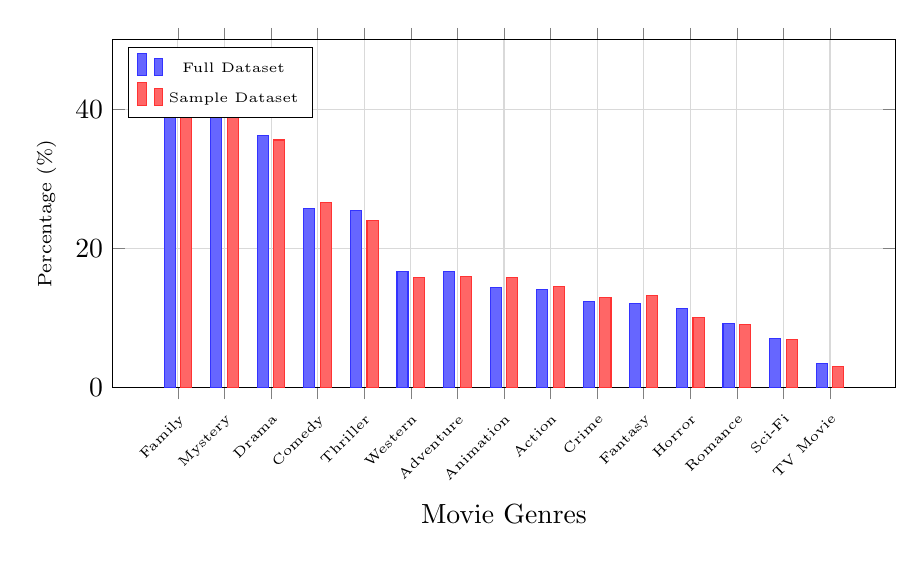
\begin{tikzpicture}
\begin{axis}[
    width=0.95\columnwidth,
    height=6cm,
    ybar,
    bar width=4pt,
    ylabel={Percentage (\%)},
    xlabel={Movie Genres},
    xticklabel style={rotate=45, anchor=north east, font=\scriptsize},
    ylabel style={font=\scriptsize},
    legend style={at={(0.02,0.98)}, anchor=north west, font=\tiny},
    xtick=data,
    ymin=0,
    ymax=50,
    grid=major,
    grid style={gray!30},
    symbolic x coords={Family, Mystery, Drama, Comedy, Thriller, Western, Adventure, Animation, Action, Crime, Fantasy, Horror, Romance, Sci-Fi, TV Movie},
    x tick label style={font=\tiny},
    enlarge x limits=0.1,
    legend entries={Full Dataset, Sample Dataset}
]
\addplot+[fill=blue!60, draw=blue!80] coordinates {
    (Family, 44.6) (Mystery, 40.0) (Drama, 36.3) (Comedy, 25.8) (Thriller, 25.5) 
    (Western, 16.7) (Adventure, 16.7) (Animation, 14.4) (Action, 14.1) (Crime, 12.4) 
    (Fantasy, 12.1) (Horror, 11.4) (Romance, 9.2) (Sci-Fi, 7.0) (TV Movie, 3.5)
};
\addplot+[fill=red!60, draw=red!80] coordinates {
    (Family, 46.8) (Mystery, 38.8) (Drama, 35.6) (Comedy, 26.6) (Thriller, 24.0) 
    (Western, 15.8) (Adventure, 16.0) (Animation, 15.8) (Action, 14.6) (Crime, 13.0) 
    (Fantasy, 13.3) (Horror, 10.1) (Romance, 9.1) (Sci-Fi, 6.9) (TV Movie, 3.1)
};
\end{axis}
\end{tikzpicture}
\caption{Genre distribution comparison between full dataset ($\sim$6k movies) and evaluation sample ($\sim$1k movies), demonstrating maintained representativeness across major movie genres.}
\label{fig:genre_distribution}
\end{figure}

\begin{figure*}[!ht]
\centering
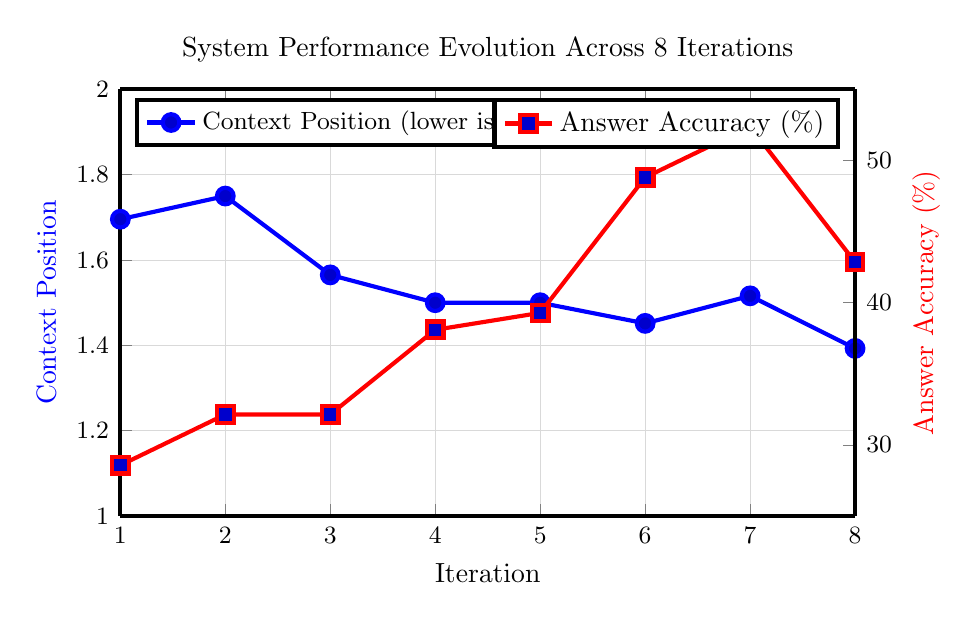
\begin{tikzpicture}
\begin{axis}[
    width=0.9\textwidth,
    height=7cm,
    xlabel={Iteration},
    ylabel={Context Position},
    ylabel style={color=blue},
    title={System Performance Evolution Across 8 Iterations},
    grid=major,
    grid style={gray!30},
    legend style={at={(0.02,0.98)}, anchor=north west, font=\small},
    xmin=1, xmax=8,
    ymin=1.0, ymax=2.0,
    xtick={1,2,3,4,5,6,7,8},
    mark size=3pt,
    line width=1.5pt,
    axis y line*=left,
    tick label style={font=\small}
]
\addplot+[color=blue, mark=*] coordinates {
    (1, 1.6957)
    (2, 1.75)
    (3, 1.5652)
    (4, 1.5)
    (5, 1.5)
    (6, 1.4516)
    (7, 1.5161)
    (8, 1.3929)
};
\addlegendentry{Context Position (lower is better)}
\end{axis}

\begin{axis}[
    width=0.9\textwidth,
    height=7cm,
    xlabel={Iteration},
    ylabel={Answer Accuracy (\%)},
    ylabel style={color=red},
    xmin=1, xmax=8,
    ymin=25, ymax=55,
    xtick={1,2,3,4,5,6,7,8},
    mark size=3pt,
    line width=1.5pt,
    axis y line*=right,
    axis x line=none,
    tick label style={font=\small}
]
\addplot+[color=red, mark=square*] coordinates {
    (1, 28.5714)
    (2, 32.1429)
    (3, 32.1429)
    (4, 38.0952)
    (5, 39.2857)
    (6, 48.8095)
    (7, 52.381)
    (8, 42.8571)
};
\addlegendentry{Answer Accuracy (\%)}
\end{axis}
\end{tikzpicture}
\caption{System performance evolution across 8 iterations showing both context position (blue line, lower is better) and answer accuracy percentage (red line). The chart demonstrates overall improvement in both metrics with context position reaching its best value at iteration 8 (1.39) and answer accuracy peaking at iteration 7 (52.38\%).}
\label{fig:iteration_performance}
\end{figure*}

\begin{table}[!t]
\centering
\small
\begin{tabularx}{\columnwidth}{lXccc}
\toprule
\textbf{Difficulty} & \textbf{Method} & \textbf{AA (\%)} & \textbf{F1} & \textbf{CA (\%)} \\
\midrule
& NF & 57.14 & 0.363 & 80.95 \\
Easy & F & 52.38 & 0.356 & 80.95 \\
& FN & 57.14 & 0.362 & 76.19 \\
\midrule
& NF & 19.04 & 0.314 & 23.81 \\
Moderate & F & 28.57 & 0.324 & 33.33 \\
& FN & 28.57 & 0.318 & 33.33 \\
\midrule
& NF & 14.28 & 0.350 & 28.57 \\
Hard & F & 19.04 & 0.356 & 33.33 \\
& FN & 23.81 & 0.316 & 38.09 \\
\midrule
& NF & 80.95 & 0.569 & n/a \\
Negative & F & 95.23 & 0.659 & n/a \\
& FN & 100.00 & 0.688 & n/a \\
\bottomrule
\end{tabularx}
\caption{RAG system performance across difficulty levels with/without metadata filter and normalization.\\
AA = Answer Accuracy, F1 = BERT F1-Score, CA = Context Accuracy;\\
NF = No Filter, F = Filtered, FN = Filtered + Normalized}
\label{tab:performance_metrics}
\end{table}

\section{Conclusion}

Our enhanced RAG system demonstrates significant improvements over baseline implementations through three key contributions: metadata filtering for targeted retrieval, query normalization for linguistic robustness, and comprehensive evaluation analytics. Evaluation across 84 gold-standard questions reveals effective performance on factual and moderate-complexity queries, with particular strength in handling temporal constraints and genre-based filtering. Quantitative results show that metadata filtering improves moderate-difficulty answer accuracy from 19.04\% to 28.57\%, while combined filtering and normalization achieves perfect 100\% accuracy on negative queries with F1-scores reaching 0.688. The iterative development process, spanning seven evaluation cycles, validates the effectiveness of prompt engineering, embedding model upgrades, and architectural modifications in addressing LLM non-determinism and retrieval accuracy challenges.

Three enhancement directions align with our development roadmap: (1) \textbf{Local Model Fine-tuning} - training specialized models on user query patterns to enable offline filter parsing, query normalization, and local embedding generation, reducing external dependencies while improving consistency in metadata extraction; (2) \textbf{Hybrid Retrieval Architecture} - combining vector search with knowledge graph representations for improved contextual understanding and relationship modeling across movie attributes; (3) \textbf{Local Answer Generation} - adapting and comparing local language models for response generation to identify optimal models for our movie question-answering use case, enabling offline operation and customizable performance tuning.

\section*{Limitations}

Our methodology faces four primary constraints that limit system capabilities and deployment scenarios: (1) \textbf{External Dependencies} - reliance on OpenAI APIs for embedding generation and language modeling creates internet connectivity requirements, subscription costs, and data privacy concerns that may restrict real-world usage scenarios; (2) \textbf{Limited Narrative Understanding} - restricted movie plot/overview data constrains character-level and narrative comprehension capabilities; (3) \textbf{Imperfect Filter Extraction} - LLM-based metadata parsing occasionally misses constraints, resulting in retrieval inconsistencies; (4) \textbf{Complex Reasoning Constraints} - inability to handle sophisticated chain-of-thought reasoning and planning for analytical queries requiring multi-step logical inference.

These limitations highlight the trade-offs between system simplicity and comprehensive question-answering capabilities in domain-specific RAG applications. While our enhancements significantly improve baseline performance, the constraints underscore ongoing challenges in building robust, production-ready RAG systems for specialized domains.

\section{Attribution}

We outline the specific contributions of each author to this research:

\textbf{Sajjad Hossain:} Led system architecture design and core RAG pipeline implementation. Developed modular data processing frameworks, metadata processing systems, and system data flow. Sourced IMDB datasets and implemented comprehensive insight generation, evaluation frameworks, analytics visualization, and prompt optimization.

\textbf{Mahmudul Hassan Navid:} Enhanced filtering capabilities and prompt engineering for metadata extraction. Designed semantic tag taxonomy and significantly contributed to gold dataset creation, validation, and system response assessment. Coordinated cross-validation of evaluation datasets.

\textbf{Md Zahidul Islam:} Conducted comprehensive sample data analysis and produced substantial portions of the gold dataset across multiple difficulty levels. Performed systematic validation of system responses, contributed to rigorous system testing, and provided critical quality assurance throughout the evaluation process.

\textbf{Nuri Jannatul:} Prepared sample datasets from full database and investigated CSV integration strategies. Contributed to gold dataset development and analyzed input data sources to establish effective data combination methodologies.

All authors participated in collaborative research conceptualization, manuscript writing, and revision processes.

\section*{Code and Data Availability}

The complete implementation and experimental resources are publicly available for reproducibility:

\begin{itemize}
\item \textbf{Repository:} \href{https://github.com/Halum/NLProc-Proj-M-SS25-team-basic/tree/develop}{\underline{GitHub repository}}
\item \textbf{Setup Guide:} \href{https://github.com/Halum/NLProc-Proj-M-SS25-team-basic/tree/develop?tab=readme-ov-file#environment-setup-with-conda}{\underline{Environment setup guide}}
\item \textbf{Gold Dataset:} \href{https://github.com/Halum/NLProc-Proj-M-SS25-team-basic/blob/develop/specialization/data/tests/gold_input_v2.json}{\underline{Evaluation dataset}}
\end{itemize}

% Bibliography section (add your .bib file reference here)
% \bibliographystyle{acl_natbib}
% \bibliography{custom}

\end{document}
